% !TeX root = 02_intro_ml_polytech.tex
% !TeX encoding = UTF-8
% !TeX spellcheck = en_GB
\begin{frame}{Linear Regression}{Let's start simple\dots}
    Let $X \in \mathbb{R}^{N \times d}$ be our \textbf{data set} and $\vec{y} = \mathbb{R}^N$ be the labels:
    \begin{equation*}
        \mathcal{D} = \left\{ (\vec{x}_i, y_i) ~\mid~ \vec{x}_i \in \mathbb{R}^d,~ y_i \in \mathbb{R} \right\}_{i = 1}^N
    \end{equation*}

    \vfill \pause

    Consider a \textbf{Linear Regression} of $y$ using the data $X$:
    \begin{equation*}
        \vec{y} = X\, \vec{\beta}
    \end{equation*}

    \textbf{Objective:} find the \enquote{best} $\vec{\beta} = (\beta_1, \beta_2, \dots, \beta_d)$ to fit the data
\end{frame}

\begin{frame}{Linear Regression}{Defining the loss function\dots}
    The \textbf{loss function} encodes a \emph{distance} between predictions and true values:

    \vfill \pause

    \begin{block}{Mean Squared Error (L2/Gauss loss)}
        \begin{equation*}
            L\left(\vec{y}, \vec{y}^{(\Theta)}\right)
            =
            \frac{1}{2N} \sum\limits_{i = 1}^N \left(y_i - y^{(\Theta)}_i\right)^2
        \end{equation*}
    \end{block}

    \begin{onlyenv}<3>
        {\tiny
        \textcolor{CEAblack!65}{%
        Since $y_i^{(\Theta)} = \sum\limits_{\ell = 1}^d X_{i, \ell}\, \beta_{\ell}$, the L2 loss is the only case where the optimal values of $\vec{\beta}$ can be computed exactly:
        \begin{equation*}
            \pdv{L\left(y, y^{(\Theta)}\right)}{\beta_{\ell}}
            =
            \frac{1}{N} \sum\limits_{i = 1}^N X_{i\ell}\, \left(y_i - X_{i\ell}\, \beta_{\ell}\right)
            =
            0
            \quad \Leftrightarrow \quad
            \sum\limits_{i = 1}^N X_{i\ell} y_i
            =
            \beta_{\ell} \left( \sum\limits_{i = 1}^N X_{i\ell} X_{i\ell} \right)
            \quad \Leftrightarrow \quad
            X^{\top} \vec{y} = \left( X^{\top} X \right) \vec{\beta}
        \end{equation*}
        which means that the coefficients are:
        \begin{equation*}
            \vec{\beta}
            =
            \left( X^{\top} X \right)^{-1} X^{\top} \vec{y}.
        \end{equation*}
        In other words, no need for gradient descent, here.
        }
        }
    \end{onlyenv}
\end{frame}

\begin{frame}{Linear Regression}{Defining the loss function\dots}
    \begin{block}{Mean Absolute Error (L1/Laplace loss)}
        \begin{equation*}
            L\left(\vec{y}, \vec{y}^{(\Theta)}\right)
            =
            \frac{1}{N} \sum\limits_{i = 1}^N \left|y_i - y^{(\Theta)}_i\right|
        \end{equation*}
    \end{block}

    \begin{block}{Mean Squared Percentage Error}
        \begin{equation*}
            L\left(\vec{y}, \vec{y}^{(\Theta)}\right)
            =
            \frac{1}{2N} \sum\limits_{i = 1}^N \left( \frac{y_i - y^{(\Theta)}_i}{y_i} \right)^2
        \end{equation*}
    \end{block}

    \begin{block}{Huber Loss}
        \small
        \begin{equation*}
            L\left(\vec{y}, \vec{y}^{(\Theta)}\right)
            =
            \frac{1}{2N} \sum\limits_{i = 1}^N \left(y_i - y^{(\Theta)}_i\right)^2\, \Theta\left( \delta - \left|y_i - y^{(\Theta)}_i\right|\right)
            +
            \frac{1}{N} \sum\limits_{i = 1}^N \left|y_i - y^{(\Theta)}_i\right|\, \Theta\left( \left|y_i - y^{(\Theta)}_i\right| - \delta \right)
        \end{equation*}
    \end{block}
\end{frame}

\begin{frame}{Constrained Optimisation}{Regularizing your models\dots}
    We saw that finding the \textbf{optimum} $\simeq$ finding equilibrium (\enquote{$\vec{F} = \vec{\nabla} L = 0$}).

    \vfill \pause

    What if we wanted to find the \textbf{optimum} in a particular situation?
    For instance:
    \begin{center}
        \emph{%
            Find the optimum of $L(\theta_1, \theta_2) = \theta_1^2 + \theta_2^2$ such that $g(\theta_1, \theta_2) = \theta_1 + \theta_2 - 1 = 0$?
        }
    \end{center}

    \vfill

    \begin{center}
        \includegraphics[height=0.4\textheight]{02_slides/img/intersecting_plane.png}
        \hfil
        \includegraphics[height=0.4\textheight]{02_slides/img/intersecting_plane_2.png}
    \end{center}
\end{frame}

\begin{frame}{Constrained Optimisation}{\includegraphics[height=12pt]{01_slides/img/tool.pdf}~Equality constraints}
    We use \textbf{Lagrange multipliers} and promote:
    \begin{equation*}
        L(\theta_1, \theta_2)
        \quad \rightarrow \quad
        \tilde{L}(\theta_1, \theta_2, \lambda)
        =
        L(\theta_1, \theta_2) + \lambda\, g(\theta_1, \theta_2)
    \end{equation*}

    \vfill \pause

    When we compute the gradient of $\tilde{L}$, we now have:
    \begin{enumerate}
        \item $\pdv{\tilde{L}}{\theta_1} = 0$ and $\pdv{\tilde{L}}{\theta_2} = 0$: these are the \enquote{old} equations (nothing changed)
        \item $\pdv{\tilde{L}}{\lambda} = 0 \Leftrightarrow g(\theta_1, \theta_2) = 0$: this condition automatically imposes the constraint!
    \end{enumerate}

    \vfill \pause

    \includegraphics[height=12pt]{01_slides/img/pen-tool.pdf}~Solve the problem from the previous slide (\emph{pen and paper})!

    \vfill \pause

    \textcolor{CEAblack!65}{%
        \begin{equation*}
            \begin{cases}
                \pdv{\tilde{L}(\theta_1, \theta_2, \lambda)}{\theta_1} & = 2 \theta_1 + \lambda = 0    \\
                \pdv{\tilde{L}(\theta_1, \theta_2, \lambda)}{\theta_2} & = 2 \theta_2 + \lambda = 0    \\
                \pdv{\tilde{L}(\theta_1, \theta_2, \lambda)}{\lambda}  & = \theta_1 + \theta_2 - 1 = 0 \\
            \end{cases}
            \Leftrightarrow
            \begin{cases}
                \theta_1 - \theta_2  & = 0 \\
                \lambda + 2 \theta_2 & = 0 \\
                \theta_1 + \theta_2  & = 1 \\
            \end{cases}
            \Leftrightarrow
            \begin{cases}
                \theta_1 & = \frac{1}{2} \\
                \theta_2 & = \frac{1}{2} \\
                \lambda  & = - 1         \\
            \end{cases}
            \Rightarrow
            L(\theta_1, \theta_2) = \frac{1}{2}.
        \end{equation*}
    }
\end{frame}

\begin{frame}{Constrained Optimisation}{What about milder constraints?}
    \begin{center}
        \emph{%
            Find the optimum of $L(\theta_1, \theta_2) = \theta_1^2 + \theta_2^2$ such that $g(\theta_1, \theta_2) = 4 - \theta_1^2 - \theta_2^2 \le 0$
        }

        {\tiny Find the minimum, but \enquote{above} the circle $\theta_1^2 + \theta_2^2 = 4$}
    \end{center}

    \vfill \pause

    We can proceed as before:
    \begin{equation*}
        \tilde{L}(\theta_1, \theta_2, \lambda)
        =
        L(\theta_1, \theta_2) + \lambda\, g(\theta_1, \theta_2)
        \alert{\quad \text{such that} \quad \lambda \ge 0}
    \end{equation*}
    and realise that
    \begin{columns}[c]
        \begin{column}{0.6\textwidth}
            \only<2>{%
                \begin{equation*}
                    (\theta_1^*, \theta_2^*, \lambda^*)
                    =
                    \arg\min\limits_{\theta_1, \theta_2}
                    \begin{cases}
                        L(\theta_1, \theta_2) & \qif g(\theta_1, \theta_2) \le 0
                        \\
                        \infty                & \qif g(\theta_1, \theta_2) > 0
                    \end{cases}
                \end{equation*}
            }
            \only<3->{%
            \begin{equation*}
                (\theta_1^*, \theta_2^*, \lambda^*)
                =
                \underbrace{%
                    \arg\min\limits_{\theta_1, \theta_2}
                    \arg\max\limits_{\lambda}
                    \tilde{L}(\theta_1, \theta_2, \lambda)
                }_{\text{saddle point!}}
            \end{equation*}
            and
            \begin{equation*}
                \lambda^*\, g(\theta_1^*, \theta_2^*) = 0
            \end{equation*}

            {\tiny Either the \alert<4>{constraint is active} and $\lambda > 0$, or the \alert<5>{constraint is satisfied} and $\lambda = 0$}
            }
        \end{column}
        \hfil
        \begin{column}{0.35\textwidth}
            \centering
            \begin{tikzpicture}
    % Axes
    \draw[thick, ->] (-0.25, 0.0) -- (3.0, 0.0) node[below] {$\theta_1$};
    \draw[thick, ->] (0.0, -0.25) -- (0.0, 3.0) node[left] {$\theta_2$};

    % Ellipses
    \draw[thin, CEAblue, fill=CEAblue!25] (1.5, 1.5) ellipse (0.75 and 1.25);
    \draw[thin, CEAgreen, fill=CEAgreen!25] (1.5, 1.5) ellipse (0.5 and 0.75);
    \draw[thin, CEAred, fill=CEAred!25] (1.5, 1.5) ellipse (0.25 and 0.25);

    % Avoid area
    \draw<3->[thin, CEAblack, fill=CEAblack!85] (1.5, 1.5) node[white] {$\infty$} circle (0.65);

    % Possible minima
    \draw<4>[CEAred, fill=CEAred!50] (1.5, 1.65) circle (2pt);
    \draw<4>[CEAred, fill=CEAred] (1.5, 2.15) circle (2pt);
    \draw<4>[CEAred, dashed, ->] (1.5, 1.70) -- (1.5, 2.05);

    \draw<5>[CEAred, fill=CEAred] (1.75, 2.5) circle (2pt);
\end{tikzpicture}

        \end{column}
    \end{columns}
\end{frame}

\begin{frame}{Constrained Optimisation}{\includegraphics[height=12pt]{01_slides/img/tool.pdf}~Inequality constraints}
    \includegraphics[height=12pt]{01_slides/img/pen-tool.pdf}~Solve the problem from the previous slide (\emph{pen and paper})!

    \vfill \pause

    \textcolor{CEAblack!65}{%
        In this scenario, the constraint is active:
        \begin{equation*}
            \footnotesize
            \begin{cases}
                \pdv{\tilde{L}(\theta_1, \theta_2, \lambda)}{\theta_1} = 2 (1 - \lambda) \theta_1 & = 0   \\
                \pdv{\tilde{L}(\theta_1, \theta_2, \lambda)}{\theta_2} = 2 (1 - \lambda) \theta_2 & = 0   \\
                4 - \theta_1^2 - \theta_2^2                                                       & \le 0 \\
                \lambda^* (4 - \theta_1^{*\, 2} - \theta_2^{*\, 2})                               & = 0
            \end{cases}
            \quad \Leftrightarrow \quad
            \begin{cases}
                \lambda^*                           & = 1                \\
                \theta_1^{*\, 2} + \theta_2^{*\, 2} & = 4                \\
                \theta_1                            & = u \in \mathbb{R} \\
                \theta_2                            & = v \in \mathbb{R}
            \end{cases}
        \end{equation*}
    }
    \begin{center}
        \begin{tikzpicture}[scale=0.6, every node/.style={scale=0.6}]
    % Values
    \draw[CEAblue, fill=CEAblue!25] (0, 0) circle (2.0);
    \draw[CEAgreen, fill=CEAgreen!25] (0, 0) circle (1.25);
    \draw[CEAred, fill=CEAred!25] (0, 0) circle (0.5);

    % Axes
    \draw[thick, CEAblack, ->] (-2.5, 0.0) -- (2.5, 0.0) node[below] {$\theta_1$};
    \draw[thick, CEAblack, ->] (0.0, -2.5) -- (0.0, 2.5) node[left] {$\theta_2$};

    % Avoid
    \draw<3->[CEAblack, fill=CEAblack!85] (0, 0) circle (0.75);
    \node<3->[CEAblack, anchor=west] at (0.4, 0.7) {$\theta_1^2 + \theta_2^2 = 4$};

    % Optima
    \draw<4->[CEAred, ultra thick, fill=none] (0, 0) circle (0.75);
\end{tikzpicture}

    \end{center}
\end{frame}

\begin{frame}{Avoid Overfitting}{Constraints as solution to your problems\dots}
    How does all this help us?

    \vfill \pause

    \includegraphics[height=12pt]{01_slides/img/brain.pdf}~Do you remember the \textbf{overfitting problem}?

    \vfill \pause

    We can avoid (partially) overfitting by constraining the parameters:
    \begin{equation*}
        L\left(\vec{y}, \vec{y}^{(\Theta)}\right)
        =
        \underbrace{\operatorname{MSE}\left(\vec{y}, \vec{y}^{(\Theta)}\right)}_{\text{\enquote{standard} loss}}
        \only<4,6->{+ \alpha\, \sum\limits_{i = 1}^d \theta_i^2}
        \only<5,6->{+ \beta\, \sum\limits_{i = 1}^d \left| \theta_i \right|}
    \end{equation*}
    \begin{itemize}
        \item<4,6-> $\sum\limits_{i = 1}^d \theta_i^2 \le \epsilon$: this is called \textbf{ridge regression} (or \emph{L2 regularisation})
        \item<5,6-> $\sum\limits_{i = 1}^d \abs{\theta_i} \le \epsilon$: this is called \textbf{lasso regression} (or \emph{L1 regularisation})
        \item<6-> both of them at the same time: this is called \textbf{elastic net} regression
    \end{itemize}
    {\footnotesize
    The idea is to avoid the \enquote{explosion} of the parameters and exploit them when they are \enquote{small}.
    }
\end{frame}

\begin{frame}{Avoid Overfitting}{How to evaluate your models?}
    Suppose we have \enquote{true values} $\vec{y}$ and \textbf{predictions} $\vec{y}^{(\Theta)}$.
    How to measure \textbf{how good} the model is?

    \vfill \pause

    \textbf{Coefficient of Determination:} (\emph{R-squared})
    \begin{equation*}
        R^2 = 1 - \frac{\sum\limits_{i = 1}^d (y_i - y_i^{(\Theta)})^2}{\sum\limits_{i = 1}^d (y_i - \mathbb{E}[y_i^{(\Theta)}])^2}
    \end{equation*}
    and others that you already know (mean squared error, mean absolute error, percentage errors, etc.).
    Take a look at \href{https://scikit-learn.org/stable/api/sklearn.metrics.html\#regression-metrics}{Scikit-learn regression metrics} for a nice list!

    \vfill \pause

    \textbf{N.B.:} Metrics computed on the training set give only a rough idea of how the model is able to fit some data.
    Only \textbf{test metrics} must be used to score the ability of the model to generalise!
\end{frame}

\begin{frame}[fragile]{Avoid Overfitting}{\includegraphics[height=12pt]{01_slides/img/tool.pdf}~Some hands-on on regression\dots}
    \begin{enumerate}
        \item \alert<2>{\includegraphics[height=12pt]{01_slides/img/pen-tool.pdf}~Create a new notebook \texttt{linear\_models.ipynb}}
        \item \alert<3>{\includegraphics[height=12pt]{01_slides/img/pen-tool.pdf}~Import the \texttt{api} module of the library \texttt{statsmodels} as \texttt{sm}}
        \item \alert<4>{\includegraphics[height=12pt]{01_slides/img/pen-tool.pdf}~Generate some random data using \texttt{numpy}}
        \item \alert<5>{\includegraphics[height=12pt]{01_slides/img/pen-tool.pdf}~Create an arbitrary \textbf{linear model} using your data and some parameters of your choice (remember to also add a column to the data for the intercept!)}
        \item \alert<6>{\includegraphics[height=12pt]{01_slides/img/pen-tool.pdf}~Split the data in training and test sets}
        \item \alert<7>{\includegraphics[height=12pt]{01_slides/img/pen-tool.pdf}~Define the \textbf{Ordinary Least Squares} model (linear model) using \texttt{sm.OLS}}
        \item \alert<8>{\includegraphics[height=12pt]{01_slides/img/pen-tool.pdf}~Fit the OLS to your data and print the summary of the results.}
        \item \alert<9>{\includegraphics[height=12pt]{01_slides/img/pen-tool.pdf}~Compute the predictions and their coefficient of determination ($R^2$)}
        \item \alert<10>{\includegraphics[height=12pt]{01_slides/img/pen-tool.pdf}~Fit a L1-regularised model and a L2-regularised model and compare the performance}
    \end{enumerate}

    \begin{onlyenv}<3>
        \begin{tikzpicture}[overlay]
            \node[set, yshift=-2em, xshift=-2em] at (current page.center) {
                \begin{notebookin}
import statsmodels.api as sm
                \end{notebookin}
            };
        \end{tikzpicture}
    \end{onlyenv}

    \begin{onlyenv}<4>
        \begin{tikzpicture}[overlay]
            \node[set, yshift=-2em, xshift=-2em] at (current page.center) {
                \begin{notebookin}
import numpy as np
X = np.random.randn(1000, 3)
                \end{notebookin}
            };
        \end{tikzpicture}
    \end{onlyenv}

    \begin{onlyenv}<5>
        \begin{tikzpicture}[overlay]
            \node[set, yshift=1em, xshift=-2em] at (current page.center) {
                \begin{notebookin}
X = sm.add_constant(X)  # or np.concat([np.ones((1000,1)), X], axis=1)
theta = np.array([-0.12, 0.05, 0.3, -0.05])
y = X @ theta + 0.5 * np.random.randn(1000)
                \end{notebookin}
            };
        \end{tikzpicture}
    \end{onlyenv}

    \begin{onlyenv}<6>
        \begin{tikzpicture}[overlay]
            \node[set, yshift=1em, xshift=-2em] at (current page.center) {
                \begin{notebookin}
X_train = X[:750]; y_train = y[:750]
X_test = X[750:]; y_test = y[750:]
                \end{notebookin}
            };
        \end{tikzpicture}
    \end{onlyenv}

    \begin{onlyenv}<7>
        \begin{tikzpicture}[overlay]
            \node[set, yshift=-2em, xshift=-2em] at (current page.center) {
                \begin{notebookin}
ols = sm.OLS(y_train, X_train)
                \end{notebookin}
            };
        \end{tikzpicture}
    \end{onlyenv}

    \begin{onlyenv}<8>
        \begin{tikzpicture}[overlay]
            \node[set, text width=30em, yshift=-4em, xshift=-2em] at (current page.center) {
                \begin{notebookin}
results = ols.fit()
print(results.summary())
                \end{notebookin}
                \includegraphics[height=0.5\textheight]{02_slides/img/summary_ols.png}
            };
        \end{tikzpicture}
    \end{onlyenv}

    \begin{onlyenv}<9>
        \begin{tikzpicture}[overlay]
            \node[set, text width=30em, yshift=-4em, xshift=-2em] at (current page.center) {
                \begin{notebookin}
from sklearn.metrics import r2_score

preds = results.predict(X_test)
r2 = r2_score(y_test, preds)
print("R-squared =", r2)
                \end{notebookin}
                \begin{notebookout}
R-squared = 0.10428474173501134
                \end{notebookout}
            };
        \end{tikzpicture}
    \end{onlyenv}

    \begin{onlyenv}<10>
        \begin{tikzpicture}[overlay]
            \node[set, text width=30em, yshift=-4em, xshift=-2em] at (current page.center) {
                \begin{notebookin}
results_l1 = ols.fit_regularized(alpha=0.05, L1_wt=1.0)
preds_l1 = results_l1.predict(X_test)
r2_l1 = r2_score(y_test, preds_l1)
results_l2 = ols.fit_regularized(alpha=0.1, L1_wt=0.0)
preds_l2 = results_l2.predict(X_test)
r2_l2 = r2_score(y_test, preds_l2)
print("R-squared (L1) =", r2_l1)
print("R-squared (L2) =", r2_l2)
                \end{notebookin}
                \begin{notebookout}
R-squared (L1) = 0.11323501063060759
R-squared (L2) = 0.12657738085806358
                \end{notebookout}
            };
        \end{tikzpicture}
    \end{onlyenv}
\end{frame}

\begin{frame}{Linear Models for Classification}{From regression to classification\dots}
    For now we worked with
    \begin{equation*}
        \vec{x} \in \mathbb{R}^{d}
        \quad \text{and} \quad
        y \in \mathbb{R}
    \end{equation*}

    But what if $y$ is \textbf{categorical}? Such as
    \begin{equation*}
        y \in \{ \text{cat}, \text{dog}, \text{elephant}, \dots \}
    \end{equation*}

    \vfill \pause

    This can happen for both \textbf{data} and \textbf{labels} and the only way is to convert it to numerical:
    \begin{equation*}
        \{ \text{cat}, \text{dog}, \text{elephant}, \dots \} \mapsto \{ 0, 1, 2, \dots \}
    \end{equation*}
    which establishes to which \textbf{class} a particular piece of data belongs.
\end{frame}

\begin{frame}{Linear Models for Classification}{From regression to classification\dots}
    What information do we get from \textbf{class} assignments?

    \vfill \pause

    \begin{center}
        Does $\vec{x}_i$ belong to class 1? Does $\vec{x}_i$ belong to class 2? etc.
    \end{center}

    \vfill \pause

    You can think of them in terms of their \textbf{one-hot encoding}:
    \begin{center}
        \begin{tikzpicture}
            \node (classes) at (0, 0) {
                \begin{tabular}{@{}c@{}}
                    \textbf{Classes} \\ \hline
                    1                \\
                    3                \\
                    2                \\
                    1                \\
                    2                \\
                    2                \\
                    \dots
                \end{tabular}
            };
            \node[right=of classes] (middle) {becomes};
            \node[right=of middle] (oh) {
                \begin{tabular}{@{}ccc@{}}
                    \textbf{Class 1} & \textbf{Class 2} & \textbf{Class 3} \\ \hline
                    1                & 0                & 0                \\
                    0                & 0                & 1                \\
                    0                & 1                & 0                \\
                    1                & 0                & 0                \\
                    0                & 1                & 0                \\
                    0                & 1                & 0                \\
                    \dots            & \dots            & \dots
                \end{tabular}
            };
        \end{tikzpicture}
    \end{center}
\end{frame}

\begin{frame}{Linear Models for Classification}{From regression to classification\dots}
    That is, with $K$ different classes
    \begin{equation*}
        \operatorname{OH}_K(y)
        =
        \begin{cases}
            1 & \qif y = k    \\
            0 & \qif y \neq k
        \end{cases}
    \end{equation*}

    \vfill \pause

    This allows us to answer
    \begin{center}
        With what probability does the \textbf{event} $\vec{x}$ belong to class $y$?
    \end{center}
    \begin{equation*}
        P(y = k \mid \vec{x})
    \end{equation*}
    {\tiny Remember the Naive Bayes Classifier of the first day?}

    \vfill \pause

    How to create a \textbf{predictive model} for $P(y = k \mid \vec{x})$?
\end{frame}

\begin{frame}{Linear Models for Classification}{Log-odds and linear models\dots}
    Let's call the \textbf{predicted probability} that an event is in class $k$ using a \textbf{model} with parameters $\Theta$:
    \begin{equation*}
        y_k^{(\Theta)} = P(y = k \mid \vec{x}, \Theta) \in [0, 1]
    \end{equation*}

    What are the \textbf{odds} that this is true?
    \begin{equation*}
        \text{logit}_k
        =
        \ln \underbrace{\frac{y_k^{(\Theta)}}{1 - y_k^{(\Theta)}}}_{\text{odds}}
        =
        \frac{\text{\enquote{This happens}}}{\text{\enquote{This does not happen}}}
        \in (-\infty, +\infty)
    \end{equation*}

    \vfill

    \includegraphics[height=12pt]{01_slides/img/brain.pdf}~What are the odds that an \textbf{unbiased} coin gives either head or tail?

    \includegraphics[height=12pt]{01_slides/img/brain.pdf}~What are the odds that an \textbf{biased} (80\% head) coin gives either head or tail?
\end{frame}

\begin{frame}{Linear Models for Classification}{Log-odds and linear models\dots}
    What is the simplest next step to define a model?
    Consider the model
    \begin{equation*}
        \text{logit}_k = f_{k, (\Theta)}(\vec{x}) = \sum\limits_{f = 1}^d x_f \underbrace{\Theta_{f\, k}}_{\text{matrix!}}
    \end{equation*}
    and let $f_{k,\, (\Theta)}$ be a \textbf{linear model}:
    \begin{equation*}
        \ln \frac{y_k^{(\Theta)}}{1 - y_k^{(\Theta)}}
        =
        f_{k,\, (\Theta)}(\vec{x})
        =
        \theta_{1k}\, x_1
        +
        \theta_{1k}\, x_2
        +
        \dots
    \end{equation*}
    This is called
    \begin{center}
        \textbf{Generalised Linear Model}
    \end{center}
    {\tiny You are not fitting a linear model on $y$, but on the log-odds, hence the \enquote{generalised}}
\end{frame}

\begin{frame}{Linear Models for Classification}{\includegraphics[height=12pt]{01_slides/img/tool.pdf}~Log-odds and linear models\dots}
    The peculiarity of the model is that $y_{(\Theta)}$ has a particular shape:

    \vfill

    \includegraphics[height=12pt]{01_slides/img/pen-tool.pdf}~Solve the previous equation for $y_{(\Theta)}$

    \vfill \pause

    \begin{columns}[c]
        \begin{column}{0.5\textwidth}
            The predictions follow a \textbf{logistic} curve (\emph{sigmoid}):
            \begin{equation*}
                y_k^{(\Theta)}
                =
                P(y = k \mid \vec{x})
                =
                \frac{1}{1 + e^{-f_{k,\, (\Theta)}(\vec{x})}}
                \in [0, 1]
            \end{equation*}
            which enables \textbf{class assignments}:
            \begin{equation*}
                \hat{y}^{(\Theta)} = k \qif y_k^{(\Theta)} > t
            \end{equation*}
            where $t \in [0, 1]$ is a choice.
        \end{column}
        \begin{column}{0.5\textwidth}
            \centering
            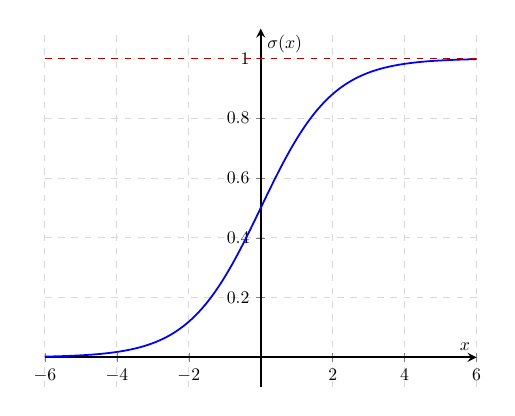
\begin{tikzpicture}[scale=0.8, every node/.style={scale=0.8}]
    \begin{axis}[
            axis lines = middle,
            xlabel = {$x$},
            ylabel = {$\sigma(x)$},
            xmin = -6, xmax = 6,
            ymin = -0.1, ymax = 1.1,
            domain = -6:6,
            samples = 100,
            smooth,
            thick,
            grid = major,
            grid style = {dashed, gray!30},
            legend pos = north west
        ]
        % Standard Logistic (Sigmoid) Function: f(x) = 1 / (1 + exp(-x))
        \addplot[color=blue] {1 / (1 + exp(-x))};

        % Asymptotic Boundaries y = 0 and y = 1
        \draw[dashed, red!70!black, thin] (axis cs:-6,1) -- (axis cs:6,1);

    \end{axis}
\end{tikzpicture}

        \end{column}
    \end{columns}
\end{frame}

\begin{frame}{Linear Models for Classification}{Multi-class classification and linear models\dots}
    What if classes are \textbf{not independent} (i.e.\ $\vec{x}$ can be $A$ or $B$, but not both)?

    \vfill

    In this case, we must also impose that the \textbf{sum of all probabilities} is 1:
    \begin{equation*}
        \sum\limits_{k = 1}^K P(y = k \mid \vec{x}) = 1
    \end{equation*}
    Hence, we get:
    \begin{equation*}
        y_k^{(\Theta)}
        =
        \frac{e^{f_{k,\, (\Theta)}(\vec{x})}}{\sum\limits_{h = 1}^K e^{f_{h,\, (\Theta)}(\vec{x})}}
        =
        \operatorname{softmax}(f_{k,\, (\Theta)}(\vec{x}))
    \end{equation*}

    \vfill \pause

    \begin{center}
        How to train a classification model?

        {\tiny \textbf{Spoiler:} it is not as simple as just comparing \enquote{errors}}
    \end{center}
\end{frame}

\begin{frame}{Linear Models for Classification}{Comparing distributions\dots}
    Suppose you have a system of particles $x \in \mathcal{X}$:
    \begin{center}
        \begin{tikzpicture}[scale=0.75, every node/.style={scale=0.75}]
    \draw[ultra thick, CEAblack] (0, 0) -- (3, 0) -- (3, 3) -- (0, 3) --cycle;

    \draw[CEAred, fill=CEAred!50] (1.0, 0.5) circle (3pt);
    \draw[CEAred, fill=CEAred!50] (1.0, 1.5) circle (3pt);
    \draw[CEAred, fill=CEAred!50] (2.0, 1.5) circle (3pt);
    \draw[CEAred, fill=CEAred!50] (2.5, 2.5) circle (3pt);
    \draw[CEAred, fill=CEAred!50] (0.5, 2.15) circle (3pt);
    \draw[CEAred, fill=CEAred!50] (0.75, 1.45) circle (3pt);
    \draw[CEAred, fill=CEAred!50] (1.75, 1.35) circle (3pt);
    \draw[CEAred, fill=CEAred!50] (0.9, 1.65) circle (3pt);
    \draw[CEAred, fill=CEAred!50] (1.2, 1.25) circle (3pt);
\end{tikzpicture}

    \end{center}
    and you want to study its distribution (its \emph{disorder}).
    You measure its entropy:
    \begin{equation*}
        H(P) = - \sum\limits_{x \in \mathcal{X}} P(x) \ln P(x) = - \mathbb{E}_P[\ln P]
    \end{equation*}

    \vfill

    And if more systems become available, you then \textbf{sum} the entropies:
    \begin{equation*}
        H_{\text{tot}}(P)
        =
        H_1(P) + H_2(P) + \dots
    \end{equation*}
\end{frame}

\begin{frame}{Linear Models for Classification}{Comparing distributions\dots}
    In this case, we have \textbf{two distributions} for \textbf{each class} (system):
    \begin{enumerate}
        \item the \textbf{true labels} $y_k \sim P$: the \textbf{one-hot} values of the labels in the data set
        \item the \textbf{predicted labels} $y_k^{(\Theta)} \sim Q$: the probabilities of belonging to class $k$
    \end{enumerate}

    \vfill

    To compare them, we use the \textbf{cross-entropy} as \textbf{loss function}:
    \begin{equation*}
        H(P, Q) = - \mathbb{E}_P[\ln Q]
        =
        - \frac{1}{N} \sum\limits_{i = 1}^N \sum\limits_{k = 1}^K y_{i,k} \ln y_{i,k}^{(\Theta)}
    \end{equation*}
    where
    \begin{equation*}
        y_{i,k} \in \{0, 1\}
        \qand
        y_{i,k}^{(\Theta)} \in [0, 1]
    \end{equation*}
\end{frame}

\begin{frame}{Linear Models for Classification}{\includegraphics[height=12pt]{01_slides/img/tool.pdf}~Comparing distributions\dots}
    \begin{enumerate}
        \item \alert<2>{\includegraphics[height=12pt]{01_slides/img/pen-tool.pdf}~Compute the cross-entropy function in the case of two classes (\emph{binary classification})}
        \item \alert<3>{\includegraphics[height=12pt]{01_slides/img/pen-tool.pdf}~Compute the gradient of the CE with respect to the parameters of the model $f_{(\Theta)}$}
    \end{enumerate}

    \vfill

    \begin{onlyenv}<2>
        If $K = 2$, then
        \begin{equation*}
            H
            =
            - \frac{1}{N}
            \sum\limits_{i = 1}^N
            \left(
            y_{i,0} \ln y_{i,0}^{(\Theta)}
            +
            y_{i,1} \ln y_{i,1}^{(\Theta)}
            \right).
        \end{equation*}
        By construction:
        \begin{equation*}
            y_{i,0} + y_{i,1} = 1
            \qand
            y_{i,0}^{(\Theta)} + y_{i,1}^{(\Theta)} = 1,
        \end{equation*}
        from which
        \begin{equation*}
            H
            =
            - \frac{1}{N}
            \sum\limits_{i = 1}^N
            \left(
            y_{i,0} \ln y_{i,0}^{(\Theta)}
            +
            (1 - y_{i,0}) \ln (1 - y_{i,0}^{(\Theta)})
            \right).
        \end{equation*}
    \end{onlyenv}

    \begin{onlyenv}<3>
        \tiny
        Consider
        \begin{equation*}
            y_{n,h}^{(\Theta)} = \frac{e^{z_{n,h}^{(\Theta)}}}{\sum\limits_{l = 1}^K e^{z_{n,l}^{(\Theta)}}}
            \qand
            z_{n,h}^{(\Theta)} = \sum\limits_{f = 1}^d X_{n\, f}\cdot \Theta_{f,\, h}.
        \end{equation*}
        Then, we can compute (\emph{chain rule})
        \begin{equation*}
            \pdv{H(\vec{y}^{(\Theta)})}{\Theta_{\ell, k}}
            =
            \sum\limits_{h = 1}^{K}
            \sum\limits_{l = 1}^{K}
            \pdv{H(\vec{y}^{(\Theta)})}{y_{n,h}^{(\Theta)}}
            \pdv{y_{n,h}^{(\Theta)}}{z_{n,l}^{(\Theta)}}
            \dv{z_{n,l}^{(\Theta)}}{\Theta_{\ell, k}}.
        \end{equation*}

        We find:
        \begin{equation*}
            \pdv{H(\vec{y}^{(\Theta)})}{y_{n,h}^{(\Theta)}}
            =
            -\frac{1}{N} \sum\limits_{n = 1}^N
            \frac{y_{n,h}}{y_{n,h}^{(\Theta)}},
            \quad
            \pdv{y_{n,h}^{(\Theta)}}{z_{n,l}^{(\Theta)}}
            =
            \frac{\delta_{lh} e^{z_{n,h}^{(\Theta)}}}{\sum\limits_{r = 1}^K e^{z_{n,r}^{(\Theta)}}}
            -
            \frac{e^{z_{n,h}^{(\Theta)}} e^{z_{n,l}^{(\Theta)}}}{\left(\sum\limits_{r = 1}^K e^{z_{n,r}^{(\Theta)}}\right)^2}
            =
            y_{n,h}^{(\Theta)} \left(\delta_{jh} - y_{n,j}^{(\Theta)}\right),
            \quad
            \dv{z_{n,j}^{(\Theta)}}{\Theta_{\ell, k}}
            =
            \delta_{jk} X_{n\, \ell}
        \end{equation*}

        Hence, we get:
        \begin{equation*}
            \pdv{H(\vec{y}^{(\Theta)})}{\Theta_{g, k}}
            =
            -
            \frac{1}{N}
            \sum\limits_{n = 1}^N
            \sum\limits_{h = 1}^{K}
            \sum\limits_{j = 1}^{K}
            \frac{y_{n,h}}{y_{n,h}^{(\Theta)}}
            y_{n,h}^{(\Theta)} \left(\delta_{jh} - y_{n,j}^{(\Theta)}\right)
            \delta_{jk} X_{n\, g}
            =
            - \frac{1}{N}
            \sum\limits_{n = 1}^N
            \left(y_{n,k} - y_{n,k}^{(\Theta)}\right) X_{n, g}
            =
            \frac{1}{N}
            \left( X^T \left( \vec{y}^{(\Theta)} - \vec{y} \right)\right)_{g k}
        \end{equation*}
        That is one component of the Gram matrix between data $X$ and the \enquote{error} $y - y^{(\Theta)}$!
    \end{onlyenv}
\end{frame}

\begin{frame}{Classification Models}{Evaluating your classification models\dots}
    How do you evaluate a classification model?

    \vfill \pause

    \begin{center}
        \begin{tikzpicture}[scale=0.5, every node/.style={scale=0.5}]
    % Bullseye
    \draw<2->[thick, CEAblack, fill=white] (0, 0) circle (4cm);
    \draw<2->[thick, CEAblue, fill=CEAblue!35] (0, 0) circle (3cm);
    \draw<2->[thick, CEAblack, fill=CEAblack!35] (0, 0) circle (2cm);
    \draw<2->[thick, CEAred, fill=CEAred!35] (0, 0) circle (1cm);
    \draw<2->[thick, CEAyellow, fill=CEAyellow!35] (0, 0) circle (0.35cm);

    % Points
    \draw<3->[CEAred, fill=CEAred!85] (1.0, 3.0) circle (3pt);
    \draw<3->[CEAred, fill=CEAred!85] (1.2, 2.75) circle (3pt);
    \draw<3->[CEAred, fill=CEAred!85] (1.1, 2.9) circle (3pt);
    \draw<3->[CEAred, fill=CEAred!85] (1.2, 3.1) circle (3pt);
    \draw<3->[CEAred, fill=CEAred!85] (1.15, 3.03) circle (3pt);
    \draw<3->[CEAred, fill=CEAred!85] (1.25, 3.23) circle (3pt);
    \draw<3->[CEAred, fill=CEAred!85] (1.05, 2.8) circle (3pt);

    % Description
    \node<3->[anchor=north] at (0, -4.25) {\huge \textbf{HIGH PRECISION}};

    \begin{scope}[xshift=9cm]
        % Bullseye
        \draw<2->[thick, CEAblack, fill=white] (0, 0) circle (4cm);
        \draw<2->[thick, CEAblue, fill=CEAblue!35] (0, 0) circle (3cm);
        \draw<2->[thick, CEAblack, fill=CEAblack!35] (0, 0) circle (2cm);
        \draw<2->[thick, CEAred, fill=CEAred!35] (0, 0) circle (1cm);
        \draw<2->[thick, CEAyellow, fill=CEAyellow!35] (0, 0) circle (0.35cm);

        % Points
        \draw<3->[CEAred, fill=CEAred!85] (0.5, 0.5) circle (3pt);
        \draw<3->[CEAred, fill=CEAred!85] (-0.5, 0.4) circle (3pt);
        \draw<3->[CEAred, fill=CEAred!85] (0.3, 0.25) circle (3pt);
        \draw<3->[CEAred, fill=CEAred!85] (-0.35, -0.5) circle (3pt);
        \draw<3->[CEAred, fill=CEAred!85] (0.4, -0.1) circle (3pt);
        \draw<3->[CEAred, fill=CEAred!85] (0.6, 0.39) circle (3pt);
        \draw<3->[CEAred, fill=CEAred!85] (-0.1, -0.2) circle (3pt);

        % Description
        \node<3->[anchor=north] at (0, -4.25) {\huge \textbf{HIGH ACCURACY}};
    \end{scope}

    \begin{scope}[xshift=18cm]
        % Bullseye
        \draw<2->[thick, CEAblack, fill=white] (0, 0) circle (4cm);
        \draw<2->[thick, CEAblue, fill=CEAblue!35] (0, 0) circle (3cm);
        \draw<2->[thick, CEAblack, fill=CEAblack!35] (0, 0) circle (2cm);
        \draw<2->[thick, CEAred, fill=CEAred!35] (0, 0) circle (1cm);
        \draw<2->[thick, CEAyellow, fill=CEAyellow!35] (0, 0) circle (0.35cm);

        % Points
        \draw<3->[CEAred, fill=CEAred!85] (0.15, 0.05) circle (3pt);
        \draw<3->[CEAred, fill=CEAred!85] (-0.05, 0.04) circle (3pt);
        \draw<3->[CEAred, fill=CEAred!85] (0.1, 0.15) circle (3pt);
        \draw<3->[CEAred, fill=CEAred!85] (-0.05, -0.2) circle (3pt);
        \draw<3->[CEAred, fill=CEAred!85] (0.05, -0.1) circle (3pt);
        \draw<3->[CEAred, fill=CEAred!85] (0.01, 0.1) circle (3pt);
        \draw<3->[CEAred, fill=CEAred!85] (-0.01, -0.05) circle (3pt);

        % Description
        \node<3->[anchor=north, text width=25em, align=center] at (0, -4.25) {\huge \textbf{HIGH ACCURACY AND HIGH PRECISION}};
    \end{scope}
\end{tikzpicture}

    \end{center}
\end{frame}

\begin{frame}{Classification Models}{Evaluating your classification models\dots}
    We thus need to define \textbf{for each class} $k = 1, \dots, K$:

    \vfill

    \begin{columns}[c]
        \begin{column}{0.3\textwidth}
            \centering
            \begin{tikzpicture}[scale=0.7, every node/.style={scale=0.7}]
    \draw[thick, CEAblack] (0, 0) rectangle (5, 5);
    \draw[thick, CEAblack] (0, 0) rectangle (5, 2.5);
    \draw[thick, CEAblack] (0, 0) rectangle (2.5, 5);

    \node[anchor=south] at (2.5, 6.1) {\textbf{CONFUSION MATRIX}};
    \node[anchor=south] at (2.5, 5.6) {\textbf{PREDICTED}};
    \node[anchor=south, rotate=90] at (-0.6, 2.5) {\textbf{ACTUAL}};

    \node[anchor=south] at (1.25, 5.1) {POSITIVE};
    \node[anchor=south] at (3.75, 5.1) {NEGATIVE};
    \node[anchor=south, rotate=90] at (-0.1, 3.75) {POSITIVE};
    \node[anchor=south, rotate=90] at (-0.1, 1.25) {NEGATIVE};

    \node[anchor=center] at (1.25, 3.75) {\huge \textbf{TP}};
    \node[anchor=center] at (3.75, 3.75) {\huge \textbf{FN}};
    \node[anchor=center] at (1.25, 1.25) {\huge \textbf{FP}};
    \node[anchor=center] at (3.75, 1.25) {\huge \textbf{TN}};
\end{tikzpicture}

        \end{column}
        \hfil
        \begin{column}{0.7\textwidth}
            \begin{itemize}
                \item \textbf{TP} {\footnotesize (\emph{true positive})}: was class $k$, predicted class $k$ (\emph{good!})
                \item \textbf{TN} {\footnotesize (\emph{true negative})}: was not class $k$, did not predict class $k$ (\emph{good!})
                \item \textbf{FN} {\footnotesize (\emph{false negative})}: was class $k$, did not predict class $k$ (\emph{missed!})
                \item \textbf{FP} {\footnotesize (\emph{false positive})}: was not class $k$,  predicted class $k$ (\emph{false alarm!})
            \end{itemize}

            \pause

            Measure accept/reject the \textbf{null hypothesis}
            \begin{center}
                $\mathcal{H}_0$: sample $\vec{x}_i$ \emph{does not} belong to class $k$
            \end{center}
            or \textbf{alternative hypothesis}
            \begin{center}
                $\mathcal{H}_1$: sample $\vec{x}_i$ belongs to class $k$
            \end{center}
        \end{column}
    \end{columns}
\end{frame}

\begin{frame}{Classification Models}{Evaluating your classification models\dots}
    \begin{columns}[c]
        \begin{column}{0.3\textwidth}
            \centering
            \begin{tikzpicture}[scale=0.7, every node/.style={scale=0.7}]
    \draw[thick, CEAblack] (0, 0) rectangle (5, 5);
    \draw[thick, CEAblack] (0, 0) rectangle (5, 2.5);
    \draw[thick, CEAblack] (0, 0) rectangle (2.5, 5);

    \node[anchor=south] at (2.5, 6.1) {\textbf{CONFUSION MATRIX}};
    \node[anchor=south] at (2.5, 5.6) {\textbf{PREDICTED}};
    \node[anchor=south, rotate=90] at (-0.6, 2.5) {\textbf{ACTUAL}};

    \node[anchor=south] at (1.25, 5.1) {POSITIVE};
    \node[anchor=south] at (3.75, 5.1) {NEGATIVE};
    \node[anchor=south, rotate=90] at (-0.1, 3.75) {POSITIVE};
    \node[anchor=south, rotate=90] at (-0.1, 1.25) {NEGATIVE};

    \node[anchor=center] at (1.25, 3.75) {\huge \textbf{TP}};
    \node[anchor=center] at (3.75, 3.75) {\huge \textbf{FN}};
    \node[anchor=center] at (1.25, 1.25) {\huge \textbf{FP}};
    \node[anchor=center] at (3.75, 1.25) {\huge \textbf{TN}};
\end{tikzpicture}

        \end{column}
        \hfil
        \begin{column}{0.7\textwidth}
            \textbf{Accuracy:}
            \begin{equation*}
                \operatorname{Acc} = \frac{\text{TP} + \text{TN}}{\text{TP} + \text{TN} + \text{FP} + \text{FN}}
            \end{equation*}
            \textbf{Precision:} (\emph{positive predicted value})
            \begin{equation*}
                \operatorname{P} = \frac{\text{TP}}{\text{TP} + \text{FP}}
            \end{equation*}
            \textbf{Recall:} (\emph{true positive rate}, \emph{sensitivity})
            \begin{equation*}
                \operatorname{R} = \frac{\text{TP}}{\text{TP} + \text{FN}}
            \end{equation*}
            \textbf{F$\beta$ Score:}
            \begin{equation*}
                \operatorname{F}_{\beta} = (1 + \beta^2) \frac{\operatorname{P} \cdot \operatorname{R}}{\beta^2 \operatorname{P} + \operatorname{R}}
            \end{equation*}
        \end{column}
    \end{columns}

    \vfill

    {\tiny See this \href{https://en.wikipedia.org/wiki/Template:Diagnostic_testing_diagram}{table} for more definitions.}
\end{frame}


\begin{frame}{Classification Models}{Evaluating your classification models\dots}
    \vfill
    \begin{columns}[c]
        \begin{column}{0.3\textwidth}
            \centering
            \begin{tikzpicture}[scale=0.7, every node/.style={scale=0.7}]
    \draw[thick, CEAblack] (0, 0) rectangle (5, 5);
    \draw[thick, CEAblack] (0, 0) rectangle (5, 2.5);
    \draw[thick, CEAblack] (0, 0) rectangle (2.5, 5);

    \node[anchor=south] at (2.5, 6.1) {\textbf{CONFUSION MATRIX}};
    \node[anchor=south] at (2.5, 5.6) {\textbf{PREDICTED}};
    \node[anchor=south, rotate=90] at (-0.6, 2.5) {\textbf{ACTUAL}};

    \node[anchor=south] at (1.25, 5.1) {POSITIVE};
    \node[anchor=south] at (3.75, 5.1) {NEGATIVE};
    \node[anchor=south, rotate=90] at (-0.1, 3.75) {POSITIVE};
    \node[anchor=south, rotate=90] at (-0.1, 1.25) {NEGATIVE};

    \node[anchor=center] at (1.25, 3.75) {\huge \textbf{TP}};
    \node[anchor=center] at (3.75, 3.75) {\huge \textbf{FN}};
    \node[anchor=center] at (1.25, 1.25) {\huge \textbf{FP}};
    \node[anchor=center] at (3.75, 1.25) {\huge \textbf{TN}};
\end{tikzpicture}

        \end{column}
        \hfil
        \begin{column}{0.7\textwidth}
            In general, used to score a classification model against the types of errors:

            \vspace{1em}

            \textbf{Type I error:} (\emph{false positive rate}, misclassification)
            \begin{center}
                \emph{How many times do I accept $\mathcal{H}_1$ even though $\mathcal{H}_0$ is true?}
            \end{center}
            \begin{equation*}
                \operatorname{FPR} = \frac{\text{FP}}{\text{TN} + \text{FP}}
            \end{equation*}

            \textbf{Type II error:} (\emph{false negative rate}, miss rate)
            \begin{center}
                \emph{How many times do I not reject $\mathcal{H}_0$ even though I should?}
            \end{center}
            \begin{equation*}
                \operatorname{FNR} = \frac{\text{FN}}{\text{TP} + \text{FN}}
            \end{equation*}
        \end{column}
    \end{columns}
    \vfill
\end{frame}

\begin{frame}{Classification Models}{\includegraphics[height=12pt]{01_slides/img/tool.pdf}Evaluating your classification models\dots}
    Consider the following ground truth labels (binary classification):
    \begin{equation*}
        y_{\text{true}}
        =
        \left[ 0, 0, 0, 1, 0, 1, 0, 1, 1, 0 \right]
    \end{equation*}
    Then, consider a model which predicts (for the same samples, in the same order):
    \begin{equation*}
        y_{\text{pred}}
        =
        \left[ 0, 1, 0, 1, 0, 1, 0, 0, 1, 1 \right]
    \end{equation*}

    \vfill

    \begin{itemize}
        \item \alert<2>{\includegraphics[height=12pt]{01_slides/img/pen-tool.pdf}~Compute the confusion matrix of the classifier}
        \item \alert<3>{\includegraphics[height=12pt]{01_slides/img/pen-tool.pdf}~Compute accuracy, precision, recall of the classifier}
        \item \alert<4>{\includegraphics[height=12pt]{01_slides/img/pen-tool.pdf}~Compute the rate of Type I and Type II errors of the classifier}
        \item \alert<5>{\includegraphics[height=12pt]{01_slides/img/brain.pdf}~Would you trust the classifier?}
    \end{itemize}

    \begin{onlyenv}<2>
        \begin{tikzpicture}[overlay]
            \begin{scope}[xshift=5cm, yshift=1cm]
                \draw[thick, CEAblack, fill=white] (0, 0) rectangle (4, 4);
                \draw[thick, CEAblack, fill=none] (0, 0) rectangle (4, 2);
                \draw[thick, CEAblack, fill=none] (0, 0) rectangle (2, 4);

                \node[anchor=south] (pred) at (2, 4.1) {\textbf{PREDICTED}};
                \node[anchor=south, rotate=90] (act) at (-0.1, 2) {\textbf{ACTUAL}};

                \node[text width=2, align=center] (tp) at (1, 3) {TP = 2};
                \node[text width=2, align=center] (fn) at (3, 3) {FN = 1};
                \node[text width=2, align=center] (fp) at (1, 1) {FP = 2};
                \node[text width=2, align=center] (tn) at (3, 1) {TN = 4};

                \begin{scope}[on background layer]
                    \node[set, fit=(tp)(fn)(fp)(fn)(pred)(act), minimum width=5cm, minimum height=5cm, xshift=0.5cm, yshift=-0.25cm] {};
                \end{scope}
            \end{scope}
        \end{tikzpicture}
    \end{onlyenv}

    \begin{onlyenv}<3>
        \begin{tikzpicture}[overlay]
            \begin{scope}[xshift=5cm, yshift=1cm]
                \node (acc) at (0, 2) {$\operatorname{Acc} = 70\%$};
                \node (prec) at (0, 1) {$\operatorname{P} = 60\%$};
                \node (rec) at (0, 0) {$\operatorname{R} = 75\%$};

                \begin{scope}[on background layer]
                    \node[set, fit=(acc)(prec)(rec), minimum width=3cm, minimum height=3cm] {};
                \end{scope}
            \end{scope}
        \end{tikzpicture}
    \end{onlyenv}

    \begin{onlyenv}<4>
        \begin{tikzpicture}[overlay]
            \begin{scope}[xshift=5cm, yshift=1cm]
                \node (fpr) at (0, 1) {$\operatorname{FPR} = 33\%$};
                \node (fnr) at (0, 0) {$\operatorname{FNR} = 25\%$};

                \begin{scope}[on background layer]
                    \node[set, fit=(fpr)(fnr), minimum width=3cm, minimum height=2cm] {};
                \end{scope}
            \end{scope}
        \end{tikzpicture}
    \end{onlyenv}
\end{frame}


\begin{frame}{Classification Models}{\includegraphics[height=12pt]{01_slides/img/tool.pdf}Evaluating your classification models\dots}
    Consider the following ground truth labels (binary classification):
    \begin{equation*}
        y_{\text{true}}
        =
        \overbrace{[ \underbrace{0, 0, 0, 0, \dots}_{999}, 1 ]}^{1000}
    \end{equation*}
    Then, consider a model which predicts (for the same samples, in the same order):
    \begin{equation*}
        y_{\text{pred}}
            =
            [ 0, 0, 0, 0, \dots ]
    \end{equation*}

    \vfill

    \begin{itemize}
        \item \alert<2>{\includegraphics[height=12pt]{01_slides/img/pen-tool.pdf}~Compute the confusion matrix of the classifier}
        \item \alert<3>{\includegraphics[height=12pt]{01_slides/img/pen-tool.pdf}~Compute the accuracy of the classifier}
        \item \alert<4>{\includegraphics[height=12pt]{01_slides/img/brain.pdf}~Would you trust the classifier?}
        \item \alert<5>{\includegraphics[height=12pt]{01_slides/img/pen-tool.pdf}~Compute the precision and recall of the classifier}
        \item \alert<6>{\includegraphics[height=12pt]{01_slides/img/pen-tool.pdf}~Compute the rate of Type I and Type II errors of the classifier}
        \item \alert<7>{\includegraphics[height=12pt]{01_slides/img/brain.pdf}~Would you trust the classifier?}
    \end{itemize}

    \begin{onlyenv}<2>
        \begin{tikzpicture}[overlay]
            \begin{scope}[xshift=5cm, yshift=1cm]
                \draw[thick, CEAblack, fill=white] (0, 0) rectangle (4, 4);
                \draw[thick, CEAblack, fill=none] (0, 0) rectangle (4, 2);
                \draw[thick, CEAblack, fill=none] (0, 0) rectangle (2, 4);

                \node[anchor=south] (pred) at (2, 4.1) {\textbf{PREDICTED}};
                \node[anchor=south, rotate=90] (act) at (-0.1, 2) {\textbf{ACTUAL}};

                \node[text width=2, align=center] (tp) at (1, 3) {TP = 0};
                \node[text width=2, align=center] (fn) at (3, 3) {FN = 1};
                \node[text width=2, align=center] (fp) at (1, 1) {FP = 0};
                \node[text width=2, align=center] (tn) at (3, 1) {TN = 999};

                \begin{scope}[on background layer]
                    \node[set, fit=(tp)(fn)(fp)(fn)(pred)(act), minimum width=5cm, minimum height=5cm, xshift=0.5cm, yshift=-0.25cm] {};
                \end{scope}
            \end{scope}
        \end{tikzpicture}
    \end{onlyenv}

    \begin{onlyenv}<3>
        \begin{tikzpicture}[overlay]
            \begin{scope}[xshift=5cm, yshift=1cm]
                \node (acc) at (0, 2) {$\operatorname{Acc} = 99.9\%$};

                \begin{scope}[on background layer]
                    \node[set, fit=(acc), minimum width=3cm, minimum height=2cm] {};
                \end{scope}
            \end{scope}
        \end{tikzpicture}
    \end{onlyenv}

    \begin{onlyenv}<5>
        \begin{tikzpicture}[overlay]
            \begin{scope}[xshift=5cm, yshift=1cm]
                \node (prec) at (0, 1) {$\operatorname{P} = \text{undefined}$};
                \node (rec) at (0, 0) {$\operatorname{R} = 0\%$};

                \begin{scope}[on background layer]
                    \node[set, fit=(prec)(rec), minimum width=3cm, minimum height=2cm] {};
                \end{scope}
            \end{scope}
        \end{tikzpicture}
    \end{onlyenv}

    \begin{onlyenv}<6>
        \begin{tikzpicture}[overlay]
            \begin{scope}[xshift=5cm, yshift=1cm]
                \node (fpr) at (0, 1) {$\operatorname{FPR} = 0\%$};
                \node (fnr) at (0, 0) {$\operatorname{FNR} = 100\%$};

                \begin{scope}[on background layer]
                    \node[set, fit=(fpr)(fnr), minimum width=3cm, minimum height=2cm] {};
                \end{scope}
            \end{scope}
        \end{tikzpicture}
    \end{onlyenv}
\end{frame}
